\documentclass{minimal}
\usepackage[a4paper, landscape]{geometry}
\usepackage{tikz}
\usetikzlibrary{matrix,fit,calc}

\begin{document}
\sffamily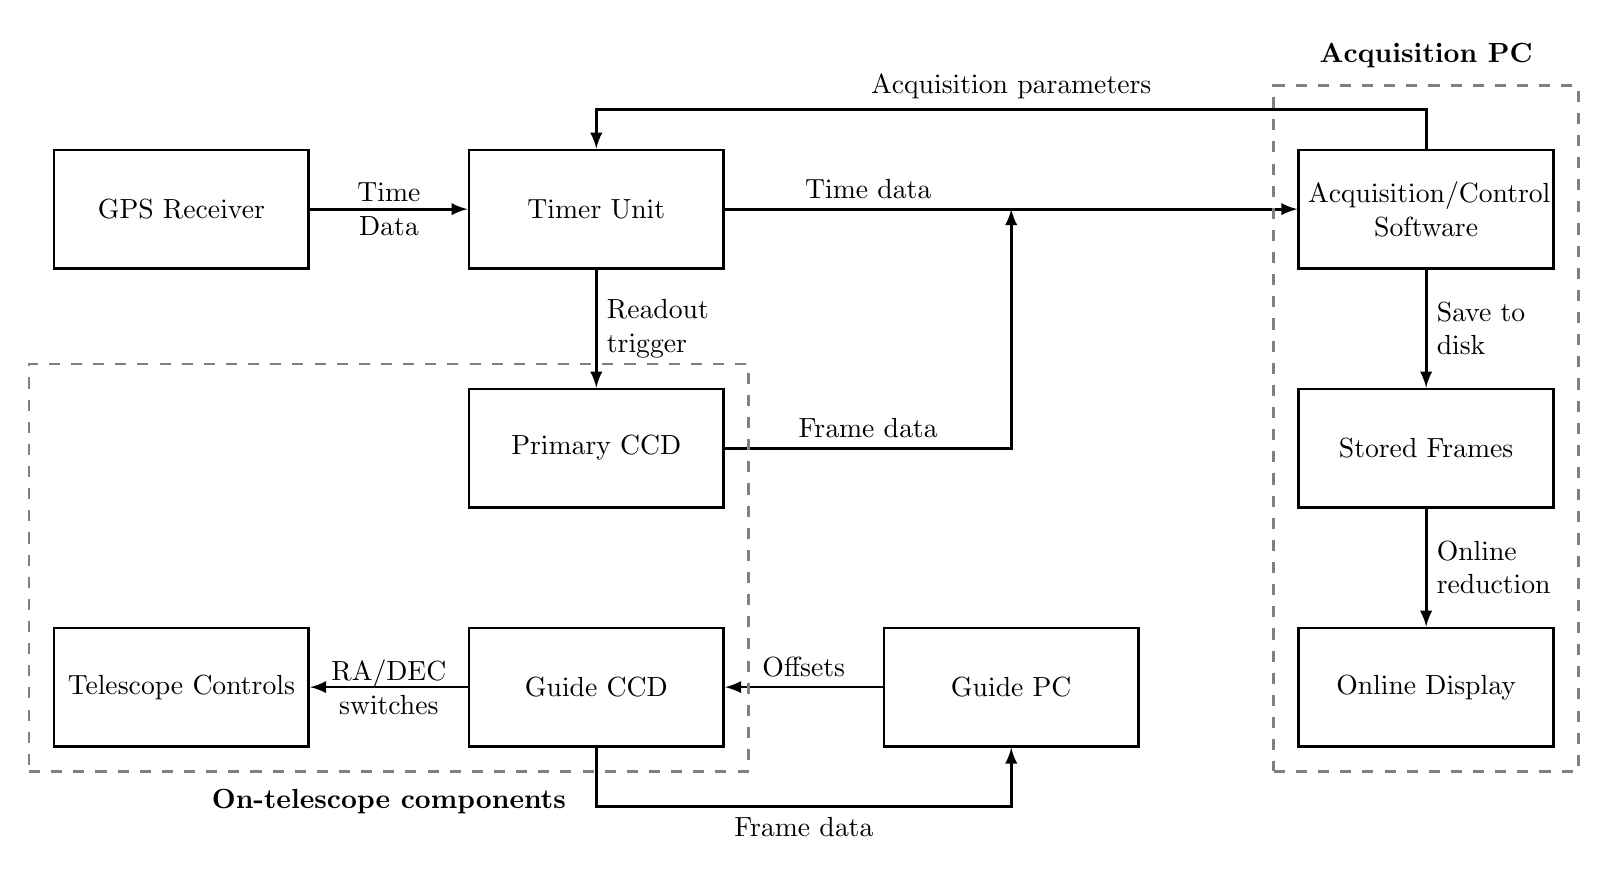
\begin{tikzpicture}
  \matrix (m) [matrix of nodes, 
    column sep=2cm,
    row sep=1.5cm,
    nodes={draw,
      line width=1pt,
      anchor=center, 
      text centered,
      minimum width=0cm, minimum height=15mm
    }, 
    txt/.style={text width=3cm,anchor=center},
    spacer/.style={draw=none},
	join/.style={draw, very thick, color=black!50, -latex'}
    ]
  {
    % m-1-1
	|[txt]| {GPS Receiver} 
  & % m-1-2
	|[txt]| {Timer Unit} 
  & % m-1-3
	|[coordinate]| {}
  & % m-1-4
	|[txt]| {Acquisition/Control Software} 
  \\
    % m-2-1
	|[spacer]| {}
  & % m-2-2
	|[txt]| {Primary CCD} 
  & % m-2-3
	|[coordinate]| {}
  & % m-2-4
	|[txt]| {Stored Frames}
  \\ 
    % m-3-1
	|[txt]| {Telescope Controls} 
  & % m-3-2
	|[txt]| {Guide CCD} 
  & % m-3-3
	|[txt]| {Guide PC} 
  & % m-3-4
	|[txt]| {Online Display}
  \\
  };

  \coordinate (m-3-2-below) at ($(m-3-2.south) + (0,-0.75cm)$) {};
  \coordinate (m-3-3-below) at ($(m-3-3.south) + (0,-0.75cm)$) {};
  \coordinate (m-1-2-above) at ($(m-1-2.north) + (0,0.5cm)$) {};
  \coordinate (m-1-4-above) at ($(m-1-4.north) + (0,0.5cm)$) {};

  {
      \path[line width=1pt, -latex] (m-1-1) edge node [align=center] {Time\\Data} (m-1-2);
      \draw[line width=1pt, -latex] (m-1-2) -- node [above, align=center] {Time data} (m-1-3) -- (m-1-4);
      \draw[line width=1pt, -latex] (m-2-2) -- node [above, align=center] {Frame data} (m-2-3) -- (m-1-3);

      \path[line width=1pt, -latex] (m-1-2) edge node [right, align=left] {Readout\\trigger} (m-2-2);
      \path[line width=1pt, -latex] (m-1-4) edge node [right, align=left] {Save to\\disk} (m-2-4);
      \path[line width=1pt, -latex] (m-2-4) edge node [right, align=left] {Online\\reduction} (m-3-4);

      \draw[line width=1pt, -latex] (m-1-4) -- (m-1-4-above) -- node [above, align=center] {Acquisition parameters} (m-1-2-above) -- (m-1-2);

      \path[line width=1pt, -latex] (m-3-2) edge node [align=center] {RA/DEC\\switches} (m-3-1);
      \path[line width=1pt, -latex] (m-3-3) edge node [above, align=center] {Offsets} (m-3-2);
      \draw[line width=1pt, -latex] (m-3-2) -- (m-3-2-below) -- node [below, align=center] {Frame data} (m-3-3-below) -- (m-3-3);
  };

  \tikzset{surround dotted/.style={draw=black!50!white, line width=1pt,
                               dash pattern=on 4pt off 4pt,
                                inner sep=3mm, rectangle}};
  
  \node (first dotted box) [surround dotted, 
                            fit = (m-1-4) (m-3-4) (m-1-4-above)] {};
  \node (second dotted box) [surround dotted,
                            fit = (m-3-1)  (m-2-2)] {};
  \node at (first dotted box.north) [above, inner sep=2mm] {\textbf{Acquisition PC}};
  \node at (second dotted box.south) [below, inner sep=2mm] {\textbf{On-telescope components}};
\end{tikzpicture}
\end{document}